\begin{figure*}[htb] {
\centering
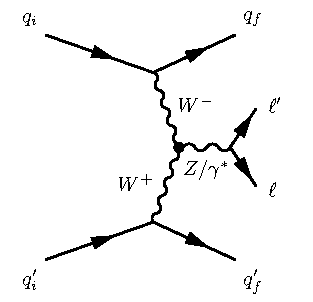
\includegraphics[width=0.315\textwidth]{figures/ss-exclboson-z2j-vbfz_diagram.pdf}
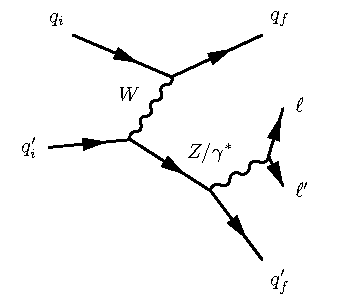
\includegraphics[width=0.35\textwidth]{figures/ss-exclboson-z2j-bckg3_diagram.pdf}
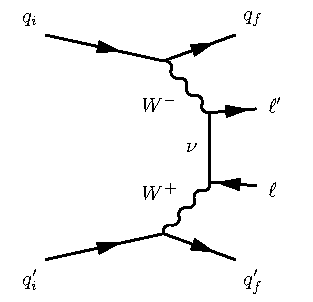
\includegraphics[width=0.315\textwidth]{figures/ss-exclboson-z2j-bckg1_diagram.pdf}
\caption{
Representative Feynman diagrams for dilepton production in association
with two jets from purely electroweak contributions:
(left) vector boson fusion,
(middle) bremsstrahlung-like,
and (right) multiperipheral production.
\label{fig:ss-exclboson-z2j-sigdiagram}}

}
\end{figure*}


\begin{figure}[p]
    \centering
    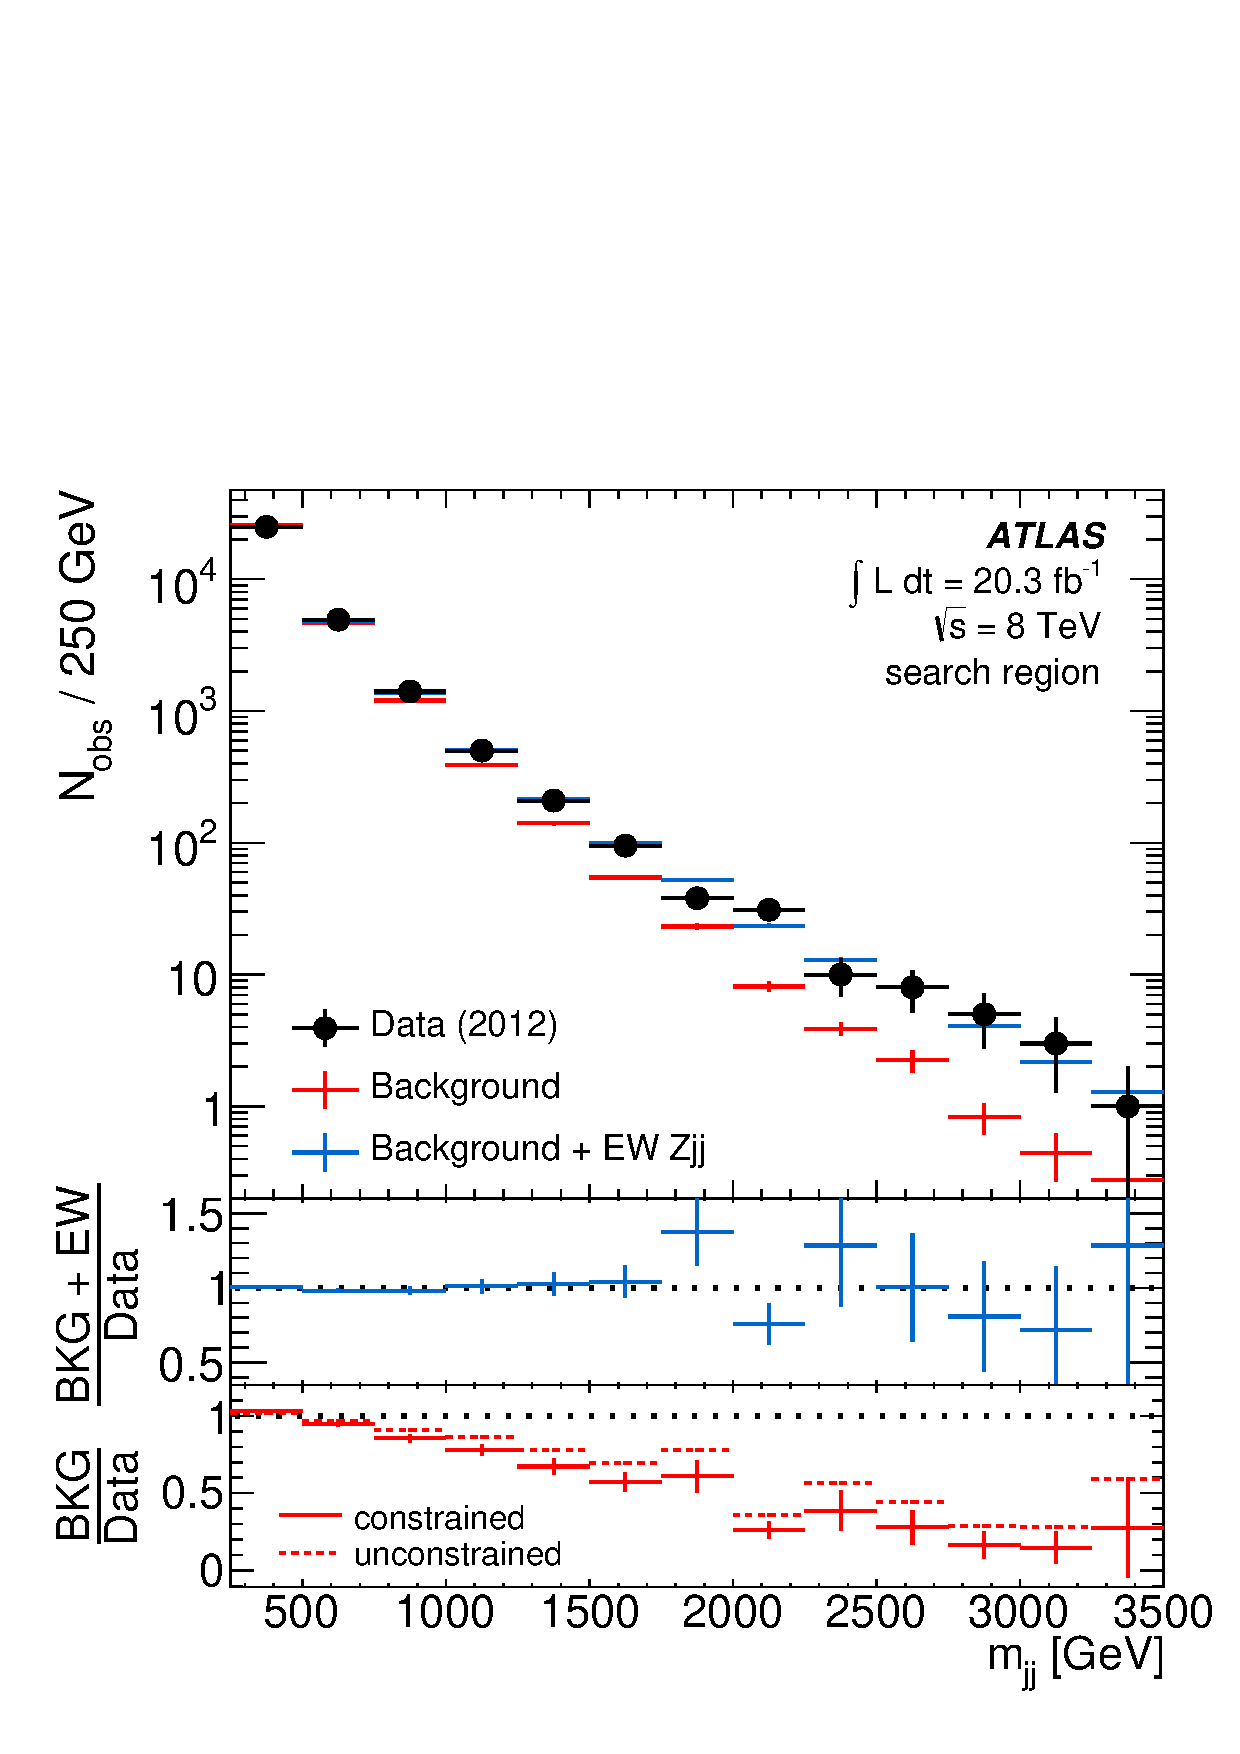
\includegraphics[width=0.45\textwidth]{figures/ss-exclboson-z2j-atlas8tev.pdf}
    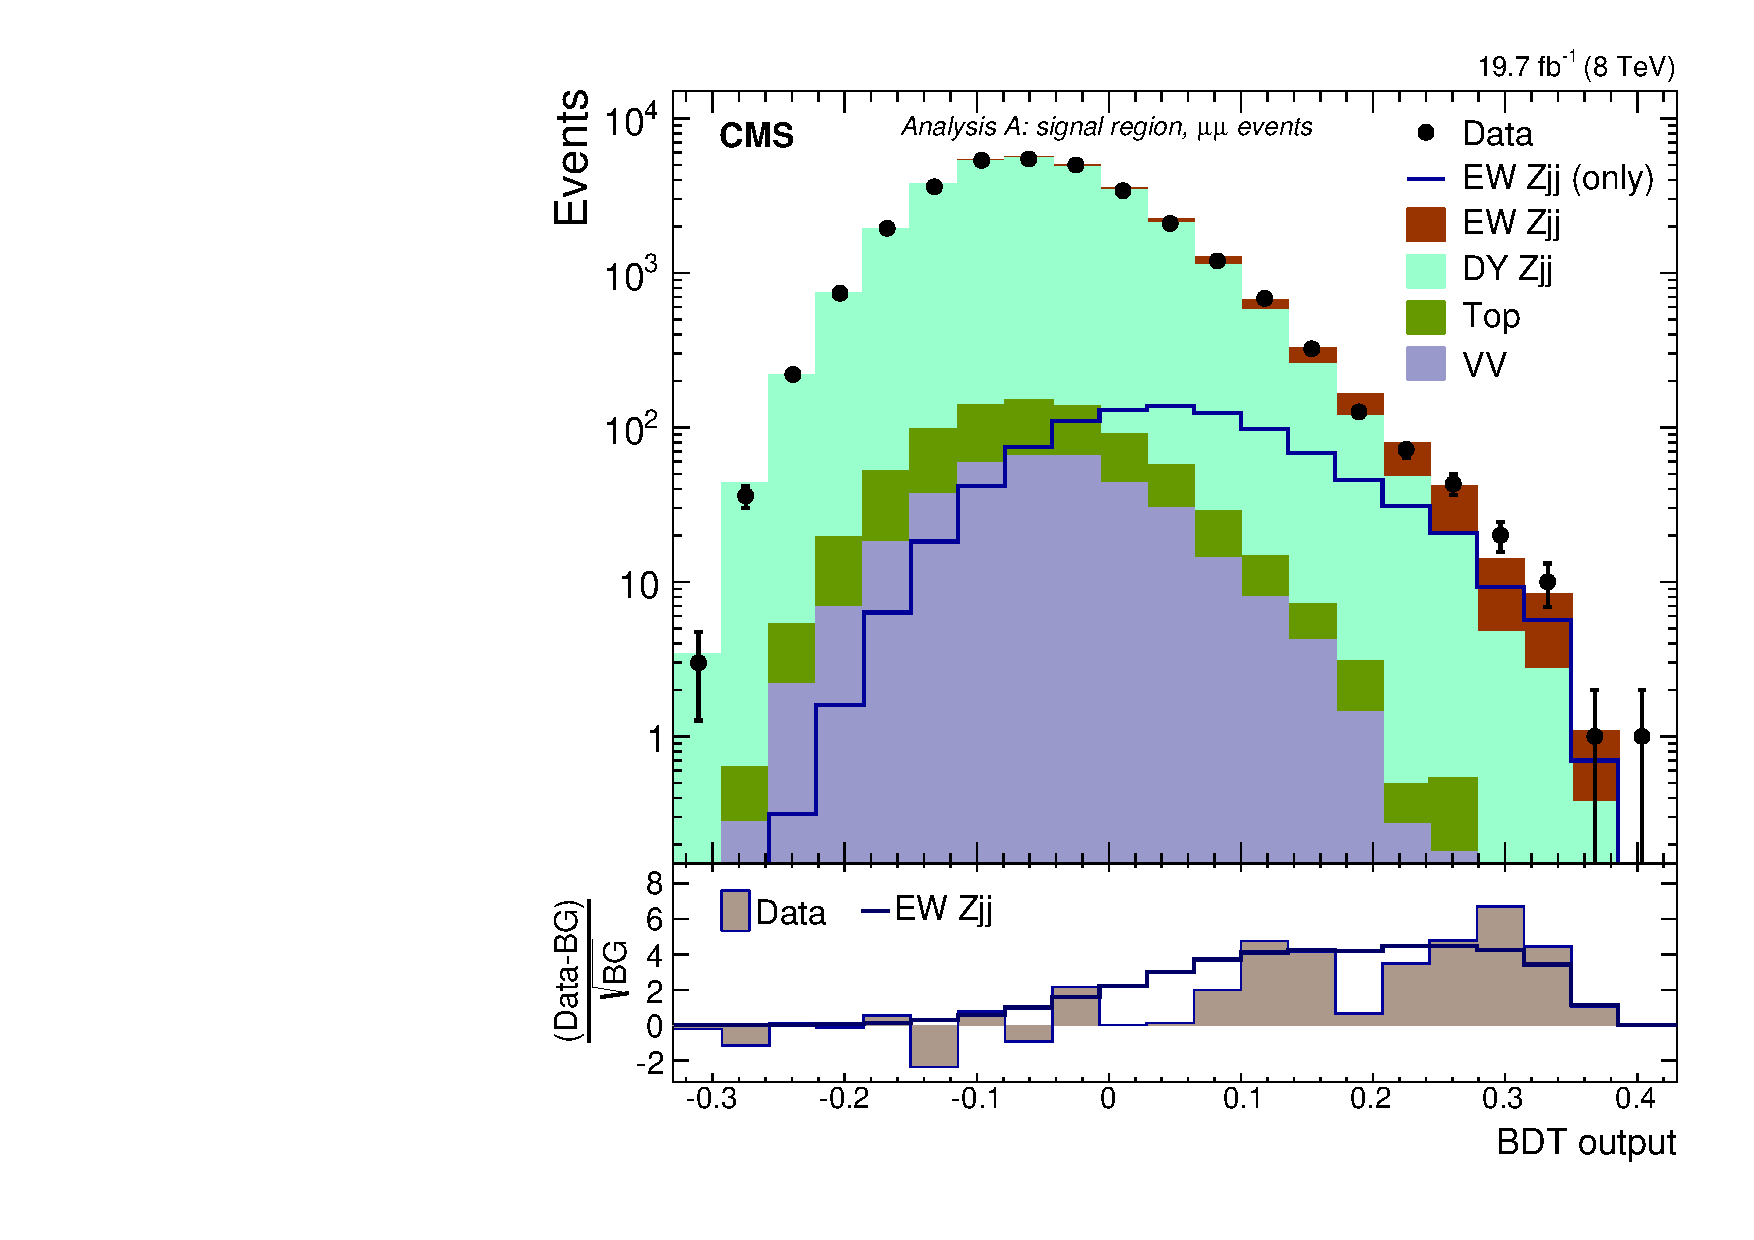
\includegraphics[width=0.45\textwidth]{figures/ss-exclboson-z2j-cms8tev.pdf}
    \caption{Evidence of observation of an electroweak amplitude in Z+2 jet production.
    Left:  The invariant mass distribution of dijets in Z+2 jet events selected
     from a signal region by ATLAS. 
    Right:  The BDT distribution of Z+2 jet events selected from a signal region
    by CMS in the dimuon channel.}
    \label{fig:ss-exclboson-z2j-8tev}
\end{figure}
ATLAS VBF Z 7 \TeV~\cite{Aad:2014dta}

CMS VBF Z 7 \TeV~\cite{Chatrchyan:2013jya}

CMS VBF Z 8 \TeV~\cite{Khachatryan:2014dea}
Figure~\ref{fig:ss-exclboson-z2j-8tev}
